%% Author_tex.tex
%% V1.0
%% 2012/13/12
%% developed by Techset
%%
%% This file describes the coding for rsproca.cls

\documentclass[openacc]{rsproca_new}%%%%where rsproca is the template name
\usepackage{subcaption}
%%%% *** Do not adjust lengths that control margins, column widths, etc. ***

%%%%%%%%%%% Defining Enunciations  %%%%%%%%%%%
\newtheorem{theorem}{\bf Theorem}[section]
\newtheorem{condition}{\bf Condition}[section]
\newtheorem{corollary}{\bf Corollary}[section]
%%%%%%%%%%%%%%%%%%%%%%%%%%%%%%%%%%%%%%%%%%%%%%%

%%%%% Please insert respective article type here %%%%
\titlehead{Research}

\begin{document}

%%%% Article title to be placed here
\title{Inferring the shape of an object inside of a tank draining of liquid through a small orifice}

\author{%%%% Author details
Gbenga Fabusola$^{1}$, 
Cory M. Simon$^{1}$
}

%%%%%%%%% Insert author address here
\address{$^{1}$School of Chemical, Biological, and Environmental Engineering. Oregon State University. Corvallis, OR, USA.
% $^{2}$Second author address\\
}

%%%% Subject entries to be placed here %%%%
\subject{applied mathematics, chemical engineering}

%%%% Keyword entries to be placed here %%%%
\keywords{inverse problems, Bayesian statistical inversion, Torricelli's law}

%%%% Insert corresponding author and its email address}
\corres{Cory M. Simon\\
\email{cory.simon@oregonstate.edu}}

%%%% Abstract text to be placed here %%%%%%%%%%%%
\begin{abstract}

\absbreak % unclear why this is needed
\end{abstract}
%%%%%%%%%%%%%%%%%%%%%%%%%%%

\rsbreak

%%%%%%%%%% Insert the texts which can accomdate on firstpage in the tag "fmtext" %%%%%

\section{Introduction}
Throughout many branches of engineering and the applied sciences, we encounter a tank draining of liquid through a small orifice, with the flow driven by gravity/hydrostatic pressure.
Mathematical models of the dynamics of the liquid level in such a tank are important for designing the geometry of the tank and orifice, predicting the emptying time, forecasting the outlet flow that may affect a process downstream, controlling the liquid level to prevent overflow or depletion, and inferring the liquid level from the outlet flow rate.

Water clocks constructed in ancient Egypt, Greece, India, and China exploited the predictable dynamics of the water level in a draining container to measure and display the passage of time. 
Specifically, the water clock (or clepsydra, Greek for ''water thief'') of the outflow design consisted of an open-top container, filled with water at some reference time, having a small aperature for outflow near its bottom. As the water drained, the elapsed time was visually indicated by the liquid level with respect to graduated markings on the inside of the container. \cite{bedini1962compartmented,hwang2021historical,ritner2016oriental,hejun1987research,schomberg2018karnak,mills1982newton}
Notably, the geometry of e.g. the preserved Karnak clepsydra from $\sim$1300 BC \cite{schomberg2018karnak}, an inverted truncated cone, does not give a constant rate of decrease in the liquid level; but, its wider top compensates for the faster outflow when the liquid level is higher.

Italian physicist and mathematician Evangelista Torricelli (1608-1647) made a fundamental observation for mathematical modeling of the liquid level in a draining tank: the velocity $v$ at which a liquid stream flows out of a small opening in a tank is proportional to the square root of the height of the liquid above the opening, $\Delta h$, i.e. $v\propto \sqrt{\Delta h}$ \cite{mills1982newton}. Today, we derive Torricelli's law from the equation of Daniel Bernoulli (1700–1782), a steady-state energy balance on the plug flow of an incompressible, inviscid fluid without frictional losses. This gives what we today refer to as \emph{Torricelli's law}: $v=\sqrt{2 g \Delta h}$, with $g$ the acceleration due to gravity. \cite{d2021torricelli} 

Combining Torricelli's law with a volume balance (assuming the liquid is incompressible) gives a first-order, [generally] nonlinear differential equation governing the dynamics of the liquid level in the tank \cite{groetsch1993inverse,seborg2016process}. The geometry of the tank comes into play through its cross-sectional area (parallel to the ground) as a function of height.
(Revisiting the outflow water clock, a container whose liquid level decreases at a constant rate as it drains may be obtained via a solid of revolution about the vertical axis with the radius scaling with the quartic root of the height. \cite{mills1982newton,d2021torricelli}) 
For quantitative agreement with the experimentally measured liquid level in a draining tank over time \cite{de2000pin,blasone2015discharge,wadhwa2021study,liu2008drainage}, we introduce a discharge coefficient $c\in (0, 1)$ and specify the outlet flow rate as $c a_o \sqrt{2 g \Delta h}$ with $a_o$ the area of the orifice. 
The discharge coefficient (i) accounts for frictional losses across the orifice, a non-uniform velocity profile, and a smaller cross-sectional area of the liquid jet than the orifice (vena contracta) and (ii) depends on the rheology of the fluid and the geometry of the orifice. \cite{teoman2022discharge,hicks2014determining,blasone2015discharge}
Finally, Torricelli's law combined with Newton's laws of motion give the trajectory of the liquid jet out of the side of the tank \cite{groetsch1999inverse}.

Modeling the liquid level in a draining tank over time and the trajectory of the liquid jet, then comparing with experiment, is an accessible, popular problem for an undergraduate physics or process dynamics course \cite{farmer1992physical,driver1998torricelli,brady2009siphons,rother2024modelling,paldy1963apparatus,ivanov2014testing,williams2021vessel,pavesi2019investigating,planinvsivc2011holes,saleta2005experimental,lopac2015water}. Draining tanks provide interesting, undergraduate-friendly inverse problems \cite{groetsch1993inverse,neto2012introduction,tarantola2005inverse} as well: inferring the liquid level in the tank from the range of the liquid jet and the shape of the tank from the liquid level measured over time \cite{groetsch1993inverse,groetsch1999inverse}.

Herein, 

\section{The forward model}

\paragraph{Tank geometry.}
We possess an open-top, plastic tank whose geometry is an inverted, right, truncated cone with a rounded rectangle as the base (and cross sections parallel to the floor). 
With $H$ [cm] the height of the tank, $a_0$ [cm$^2$] and $a_1$ [cm$^2$] the area of the rounded rectangle forming the bottom and top, respectively, of the tank, the cross-sectional area [parallel to the ground] of the tank as a function of height $h$ [cm] from the ground is:
\begin{equation}
a_t(h) = \frac{h}{H}a_1 + \left(1-\frac{h}{H}\right) a_0.
\end{equation}

\paragraph{Object inside tank.} Suppose also that a heavy (denser than water), solid (thus displaces water) object is resting inside the tank. Let $a^\prime(h)$ be the cross-sectional [parallel to the floor] area of this object as a function of height $h$. 

\paragraph{Orifice in tank.} We drilled a a small hole of radius $r_o$ [cm] in the side of the tank, holding the drill bit parallel to the floor, a height $h_o$ [cm] from the ground. 

\paragraph{Torricelli's law.} Given the height of water in the tank is $h$ [cm], we wish to model the velocity $v$ [cm/s] of the jet of water flowing out of the orifice of the tank. This outflow is driven by gravity exerting a force on the water above the orifice, which creates a hydrostatic pressure in the water at the orifice. 
Treating the water as inviscid and incompressible and the flow through the orifice as at steady-state, plug, and without frictional losses, Bernoulli's equation \cite{welty2020fundamentals}, a mechanical energy balance, simplifies to Torricelli's law \cite{d2021torricelli}:
\begin{equation}
	v =  \sqrt{2 g(h-h_o)}, \label{eq:Toricelli}
\end{equation} where $g$ [cm/s$^2$] is the acceleration due to gravity. In short, with $\rho$ [g/cm$^3$] the constant density of the water, the hydrostatic pressure in the water at the orifice, $\rho g(h-h_o)$, is relieved to give the water a kinetic energy (per mass), $\rho v^2/2$.

\paragraph{Dynamic model of the liquid height in the tank.} Now, suppose we fill the tank to an initial liquid height $h_0 \leq H$ [m] at time $t=0$ [s] then allow it drain through the orifice without further input of liquid. We wish to model the height of liquid in the tank as a function of time, $h=h(t)$, with $t$ [s] time. 
A mass balance on water for $t\geq 0$, with the tank serving as the control volume, gives:
\begin{equation}
	\frac{d}{dt} \left ( \rho V(t) \right) = - \rho c \pi r_o^2 \sqrt{2 g(h(t)-h_o)},
\end{equation}
with $c\in(0,1)$ the discharge coefficient \cite{lienhard1984velocity,hicks2014determining,wadhwa2021study,teoman2022discharge} to account for frictional losses in the flow through the orifice, the vena contracta of the liquid jet out of the tank, and the non-uniform flow profile through the orifice. The term on the right is the mass flow rate of water out of the tank, and $V(t)$ [cm$^3$] is the volume of water in the tank at time $t$. 
Since the flow rate of liquid out of the tank is small, we can treat the top of the liquid as flat and relate $V(t)$ to the height of the liquid as: 
\begin{equation}
	V(t)=\int_0^{h(t)} [a(y) - a^\prime(y)]dy,
\end{equation}
bringing the geometry of the tank and the object inside of it into play. Finally, treating the water as incompressible (constant $\rho$) gives a nonlinear, first-order differential equation for $h(t)$ subject to an initial condition:

\begin{align}
& [a_t(h)-a^\prime(h)]\frac{dh}{dt}= -c \pi r_o^2 \sqrt{2g (h(t)-h_o)}, \,\,\, t \geq 0 \\
& h(0)=h_0.
\end{align}

We refere to this as the fowardmodel bc

\section{Results}

\begin{figure}[h!]
    \centering
        \begin{subfigure}[b]{0.3\textwidth}
    	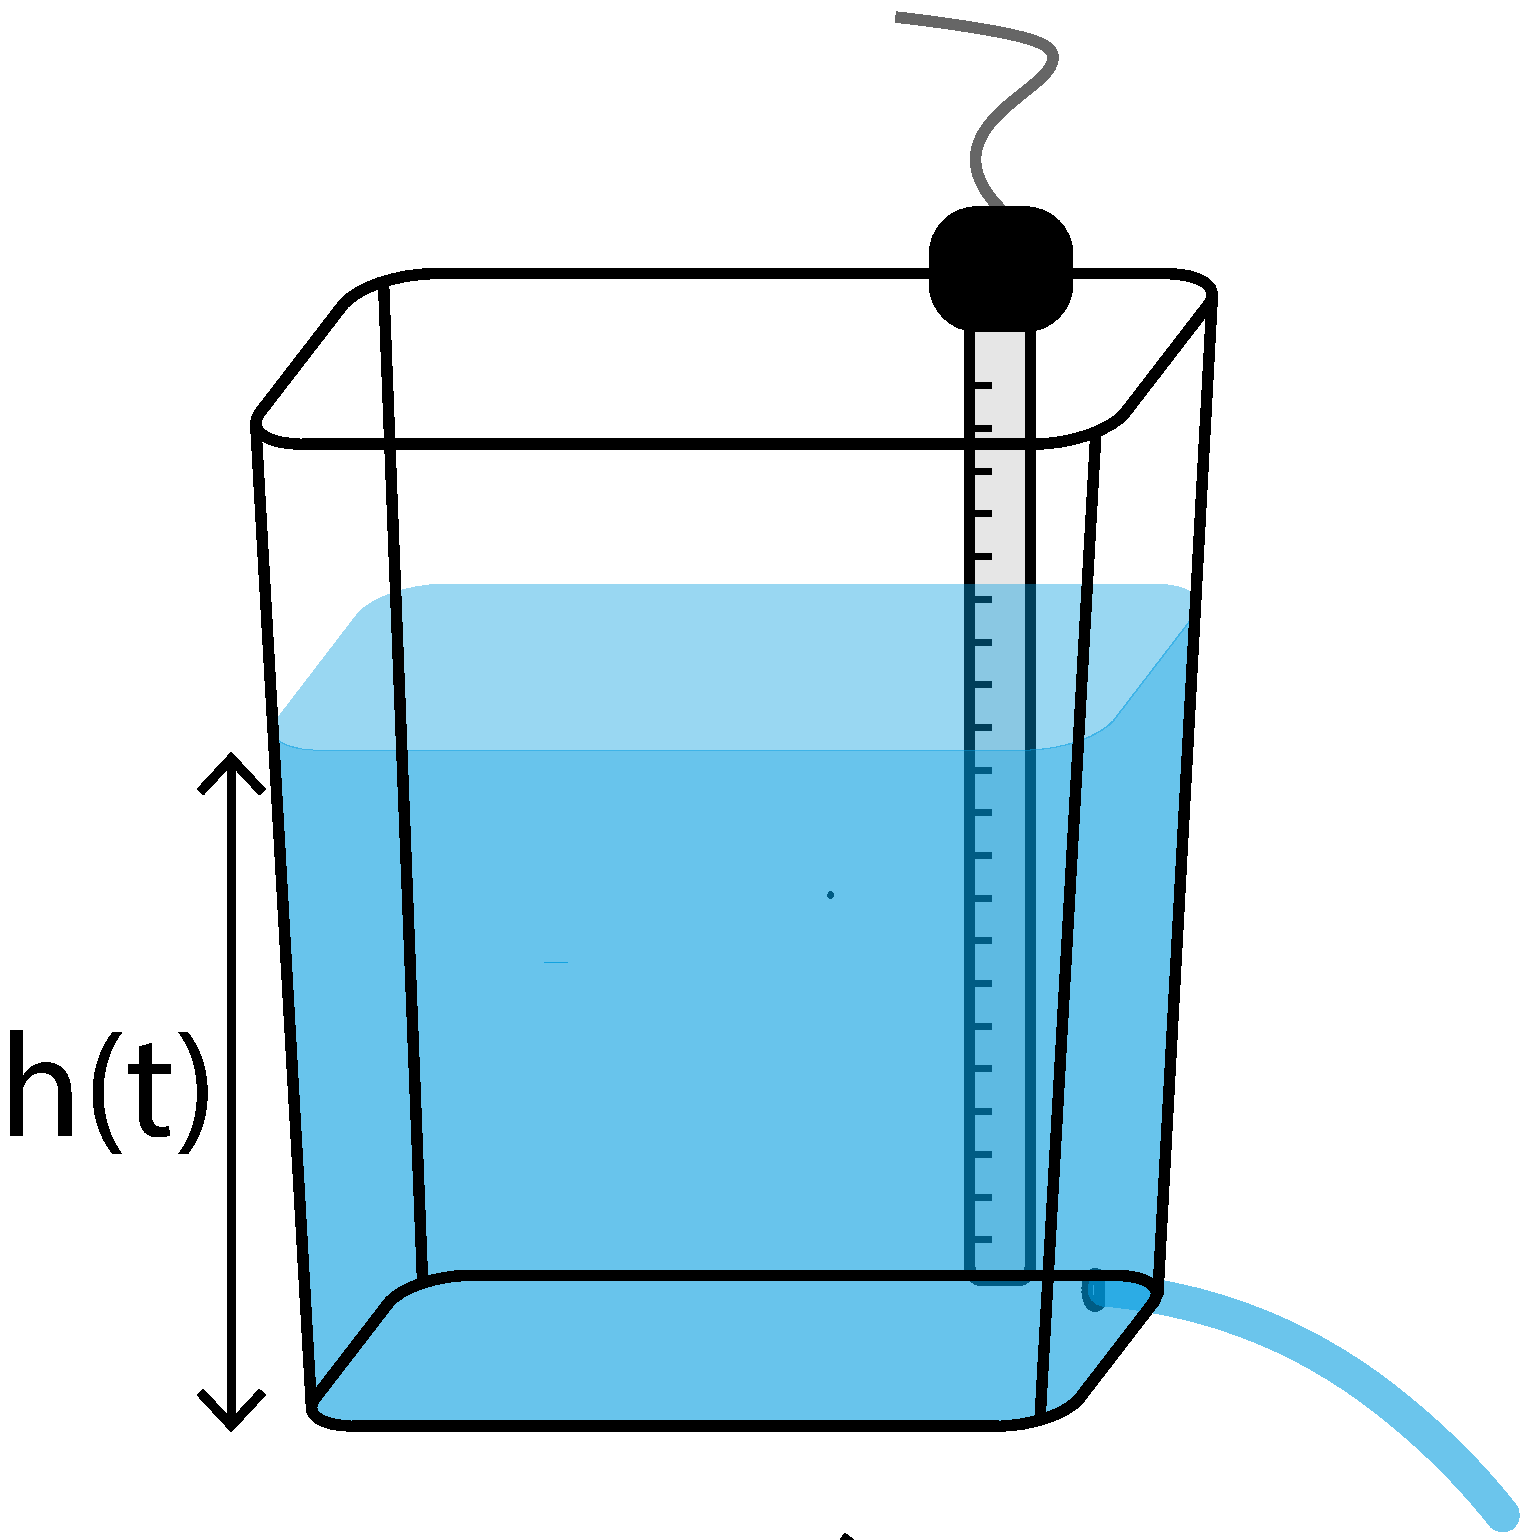
\includegraphics[width=\textwidth]{../tank_geometry/naked_tank.pdf}
	\caption{Experimental setup} \label{fig:naked_tank}
    \end{subfigure}
    
     \begin{subfigure}[b]{0.49\textwidth}
    	\includegraphics[width=\textwidth]{../prior_train.pdf}
	\caption{Prior distribution} \label{fig:prior_train}
    \end{subfigure}
     \begin{subfigure}[b]{0.49\textwidth}
    	\includegraphics[width=\textwidth]{../posterior_train.pdf}
	\caption{Data and posterior distribution} \label{fig:posterior_train}
    \end{subfigure}
    
     \begin{subfigure}[b]{0.49\textwidth}
    	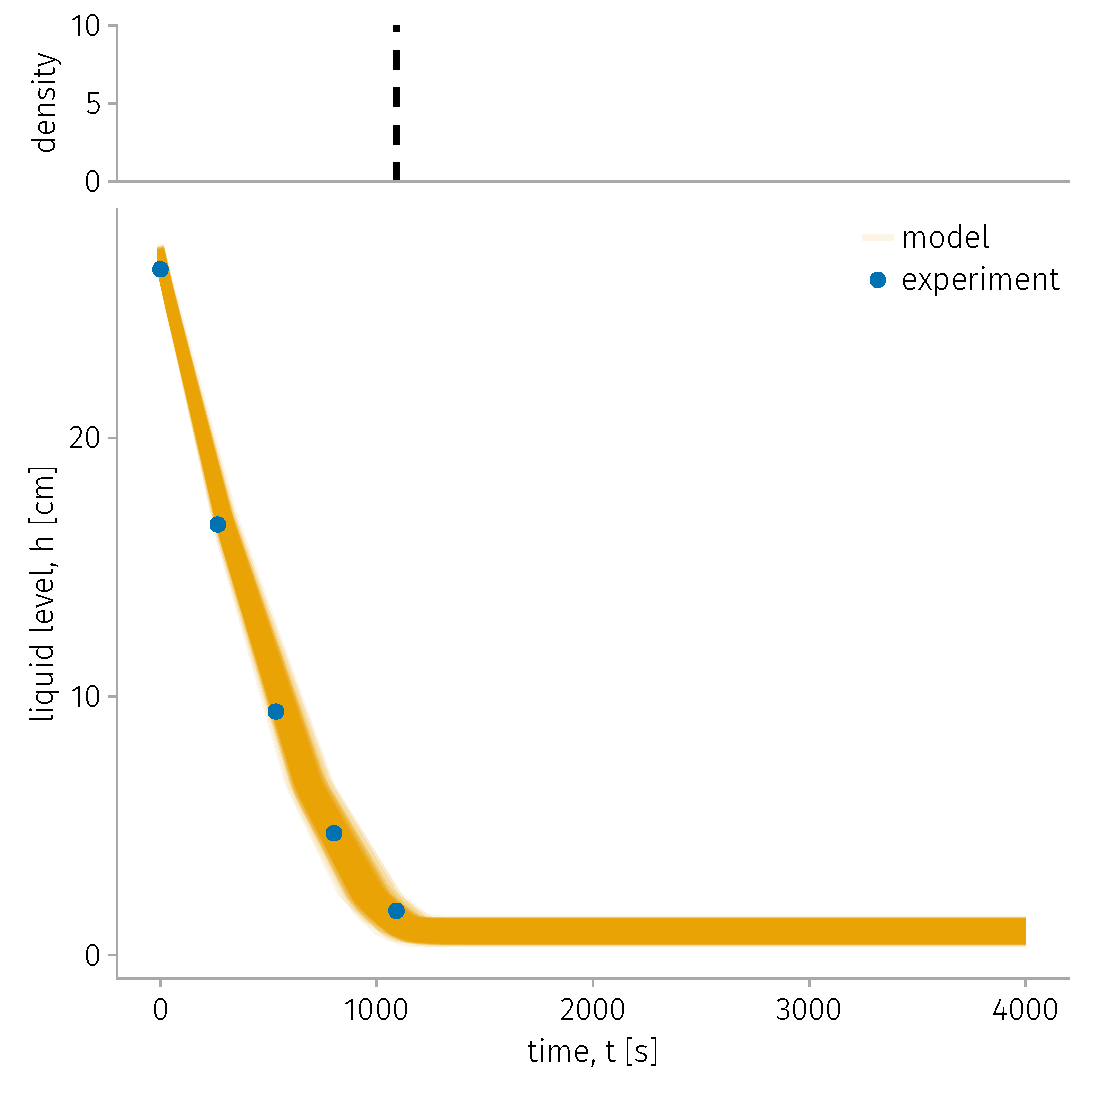
\includegraphics[width=\textwidth]{../test.pdf}
	\caption{Test} \label{fig:test}
    \end{subfigure}
    \caption{
      \textbf{Model calibration.}
      }
\end{figure}

\section{Discussion}

Mariotte's bottle \cite{kirevs2006mariotte}

\enlargethispage{20pt}

\ack{GF acknowledges ARMI for funding.}


%%%%%%%%%% Insert bibliography here %%%%%%%%%%%%%%

\vskip2pc


\bibliographystyle{RS} %%%% .BST file

\bibliography{refs} %%%%% .Bib file

\end{document}
